\section{Resultados}

\begin{frame}{Implementaci\'on del Algoritmo Propuesto (OE 2)}
    \begin{itemize}
        \item Pre y post procesamiento de resultados en {\tt Python}: 
        \begin{itemize}
            \item Pre: Extracci\'on de un grafo (JSON), a partir de una imagen (PNG),  mediante {\tt sknw}/{\tt NetworkX}
            \item Post: Visualizaci\'on de resultados
        \end{itemize}
        
        \item Algoritmo Propuesto en {\tt C++}. Par\'ametros de entrada:
        \begin{itemize}
            \item Imagen a analizar (PNG) y el grafo (JSON)
            \item Tipo de c\'elula
            \item Color del fondo/segundo plano
            \item Opcionales: Nivel de debugging
        \end{itemize}
        
        
    \end{itemize}
\end{frame}

\begin{frame}{Metodolog\'ia}
\begin{itemize}
    \item M\'etricas y Medidas: VI, \'Indice Rand, \'Indice Jaccard
    \item {\it Precision}, {\it Recall}, F1
    \item N$\degree$ Filamentos Propuestos vs {\it Ground Truth}
    \item N$\degree$ Filamentos Correctos vs {\it Ground Truth}
    \item Promedio de 5 Iteraciones del algoritmo propuesto, con distinta semillas
    \item 8 Im\'agenes: 2 Sint\'eticas, 3 de Microt\'ubulos en {\it Arabidopsis Marchantia} y 3 de neuronas de rat\'on
\end{itemize}
\end{frame}

\begin{frame}{Par\'ametros del Algoritmo Propuesto (AP) (OE 3)}
    \centering
    \begin{table}[h]
    %\centering
    \begin{tabular}{|c|c|c|c|c|}
        \hline
        & 
        & 
        \multirow{4}{1.5cm}{\it Max Axial Displ.} & \multirow{4}{1.5cm}{Permite Superposici\'on} &
        \multirow{4}{2cm}{Aplica Heur\'istica Asignaci\'on Completa}\\
        \diagbox[width=10em]{C\'elula}{Par\'ametro} & 
        $\theta$ & & &\\
        & & & &\\
         \hline
        Neurona (AP N) & 45\textdegree & 2 & Si & No\\
        MT Planta (AP MT-P) & 30\textdegree & 1.5 & Si & Si\\
        MT Animal (AP MT-A) & 60\textdegree & 2.5 & Si & Si\\
        Sint\'etico (AP S) & 45\textdegree & 1.5 & Si & No \\
        \hline
    \end{tabular}
\end{table}
\end{frame}

\begin{frame}{Ponderaci\'on de los par\'ametros (OE 3)}
    \begin{itemize}\fontsize{9pt}{12}\selectfont
    \item No es posible utilizar un \'unico par\'ametro para obtener una ponderaci\'on directa
    \item Construcci\'on de soluciones: $\frac{100}{n}$\% el grado de los nodos, y el remanente para el \'angulo entre aristas, con $n$ como el n\'umero de aristas.
    \item M\'etodo de b\'usqueda no local: 100\% posici\'on de la arista.
    \item Actualizaci\'on de feromonas: 
    \begin{itemize}\fontsize{9pt}{12}\selectfont
        \item Caso General: 50\% curvatura, 50\% diferencia de magnitud entre segmentos
        \item Neuronas: $33.\overline{3}\%$ curvatura, $33.\overline{3}\%$ diferencia de magnitud entre segmentos y $33.\overline{3}\%$ informaci\'on topol\'ogica de centralidad.
    \end{itemize}
\end{itemize}
\end{frame}

% \begin{frame}{Im\'agenes Sint\'eticas}

%     \begin{figure*}[h]
%         \centering
%         \begin{subfigure}[t]{0.31\textwidth}
%             \centering
%             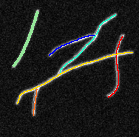
\includegraphics[height=1.3in]{Pictures/Synth-QuantitativeIFS-Fig7_groundTruth.png}
%         \end{subfigure}
%         ~ %\hspace{0.1cm}
%         \begin{subfigure}[t]{0.31\textwidth}
%             \centering
%             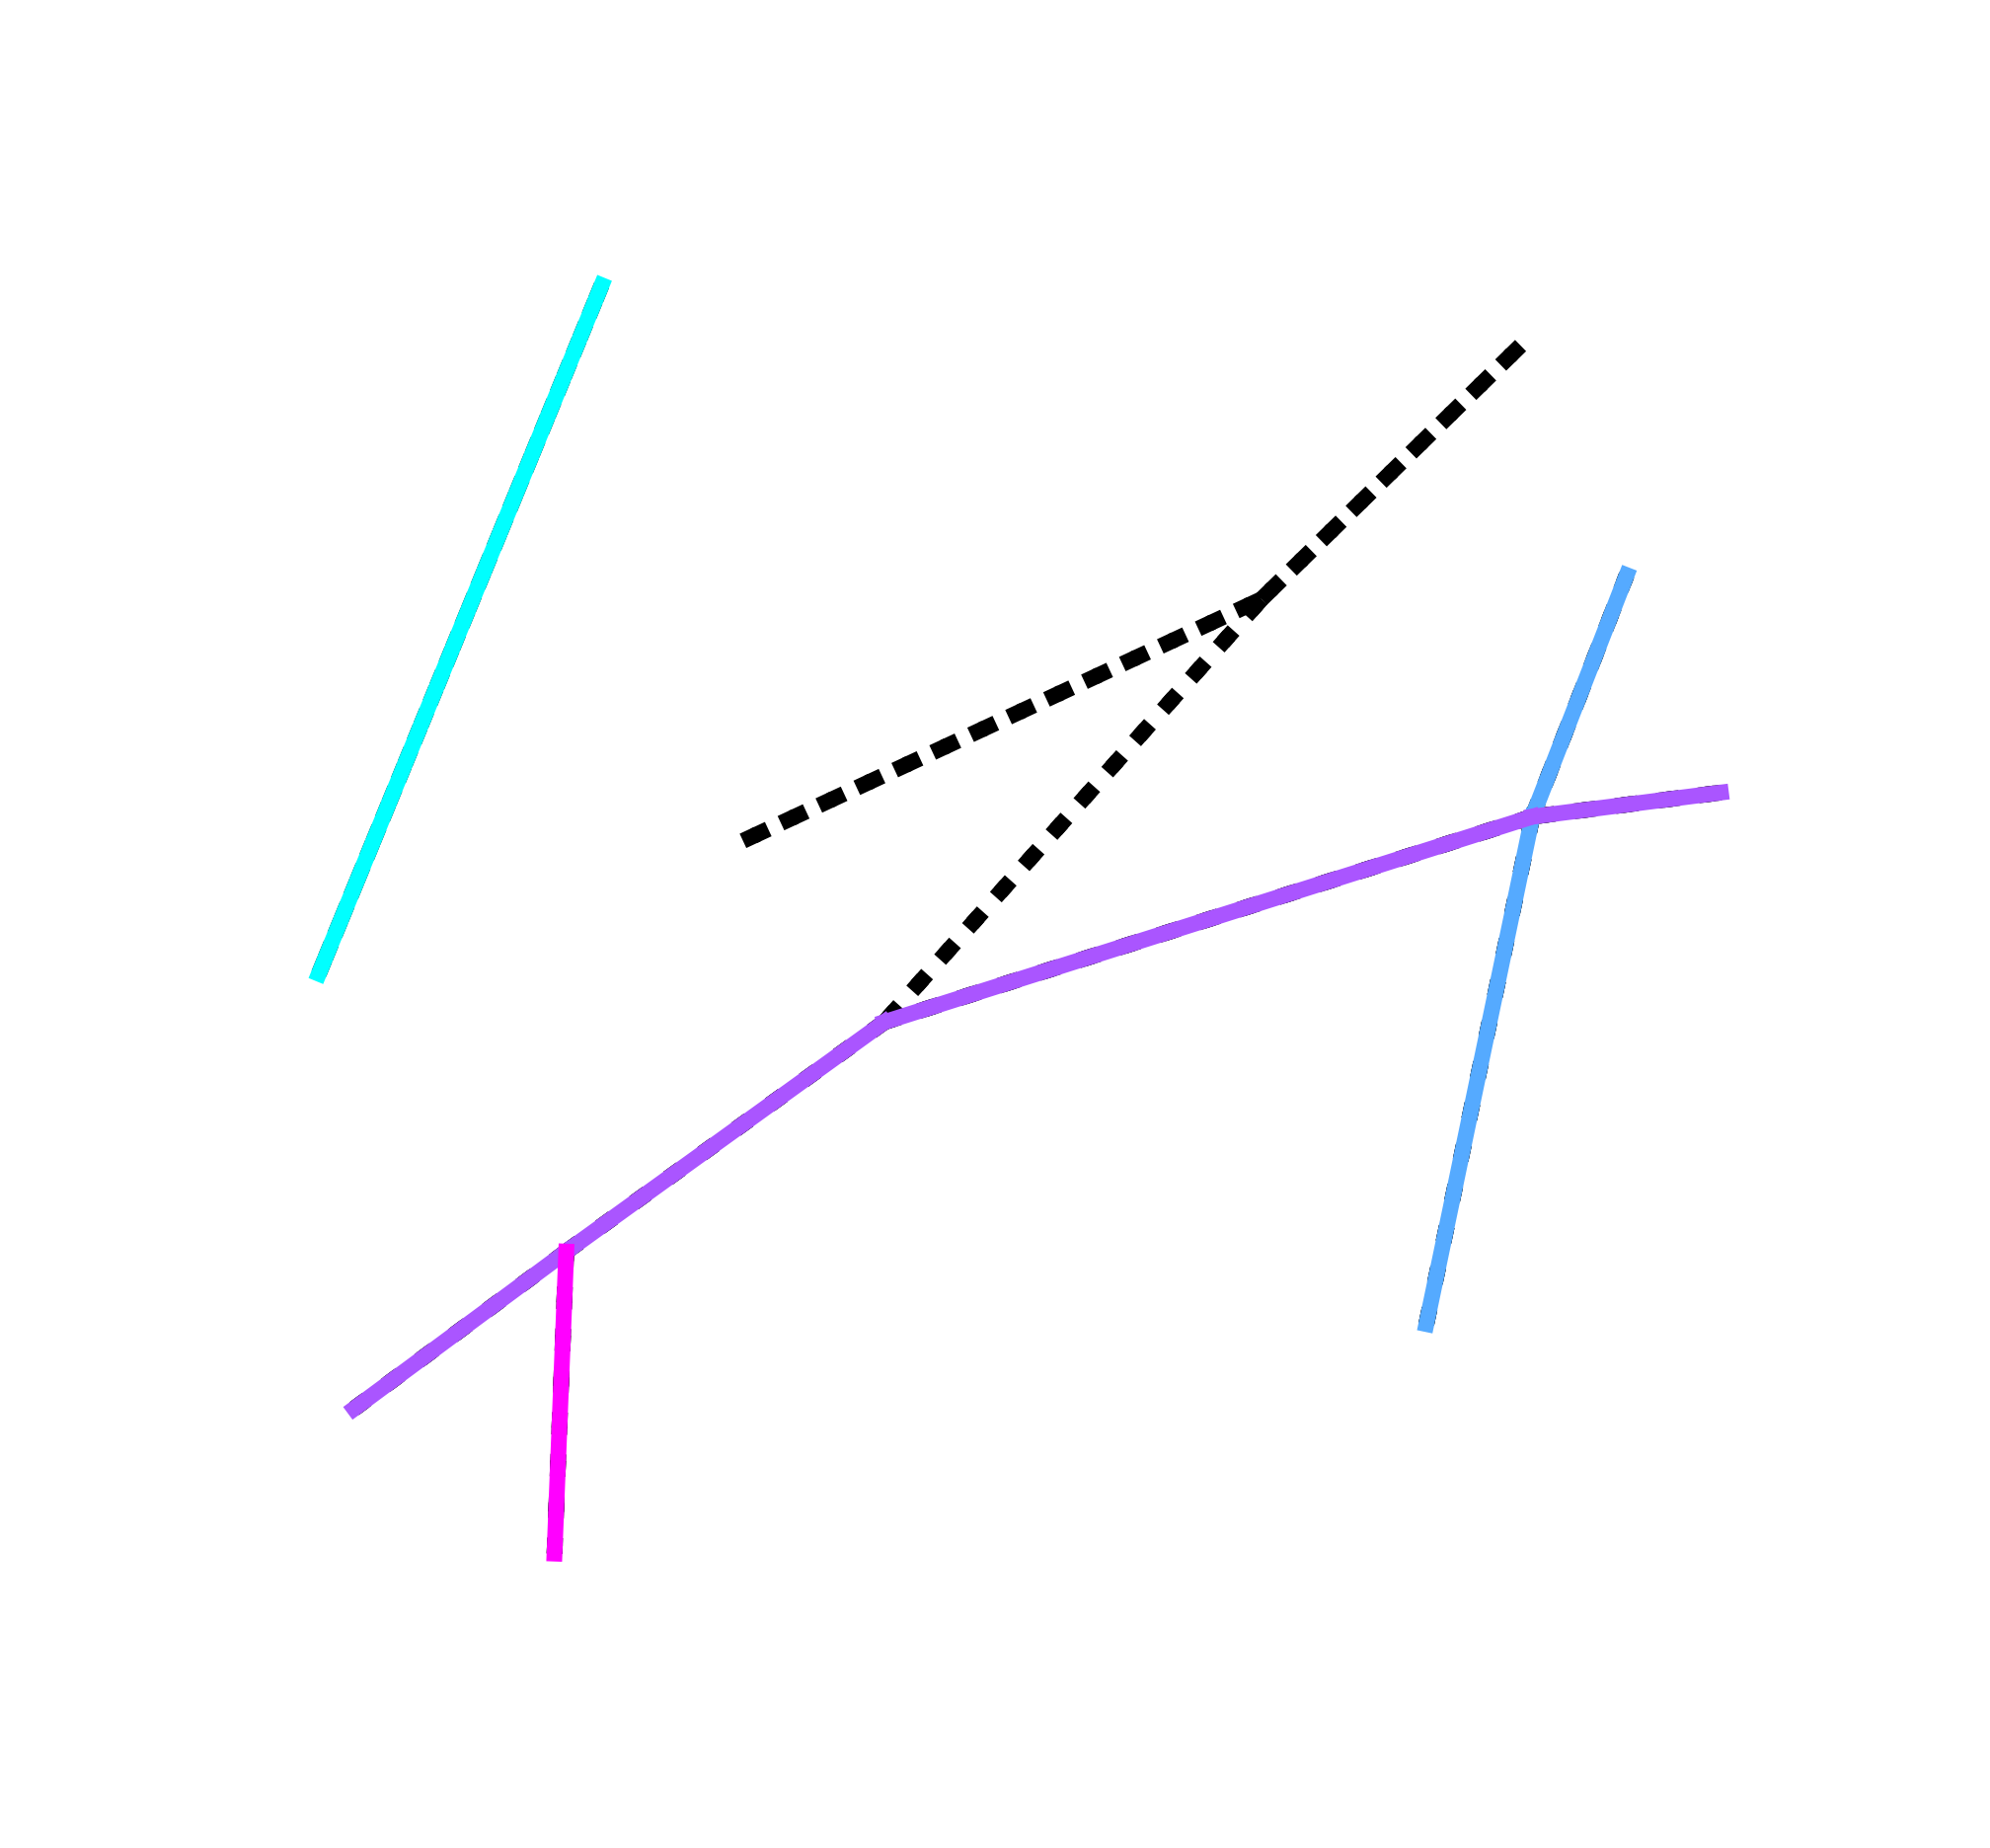
\includegraphics[height=1.3in]{Pictures/QFS7-DeFiNeExactMatch-30.png}
%         \end{subfigure}
%         ~
%         \begin{subfigure}[t]{0.31\textwidth}
%             \centering
%             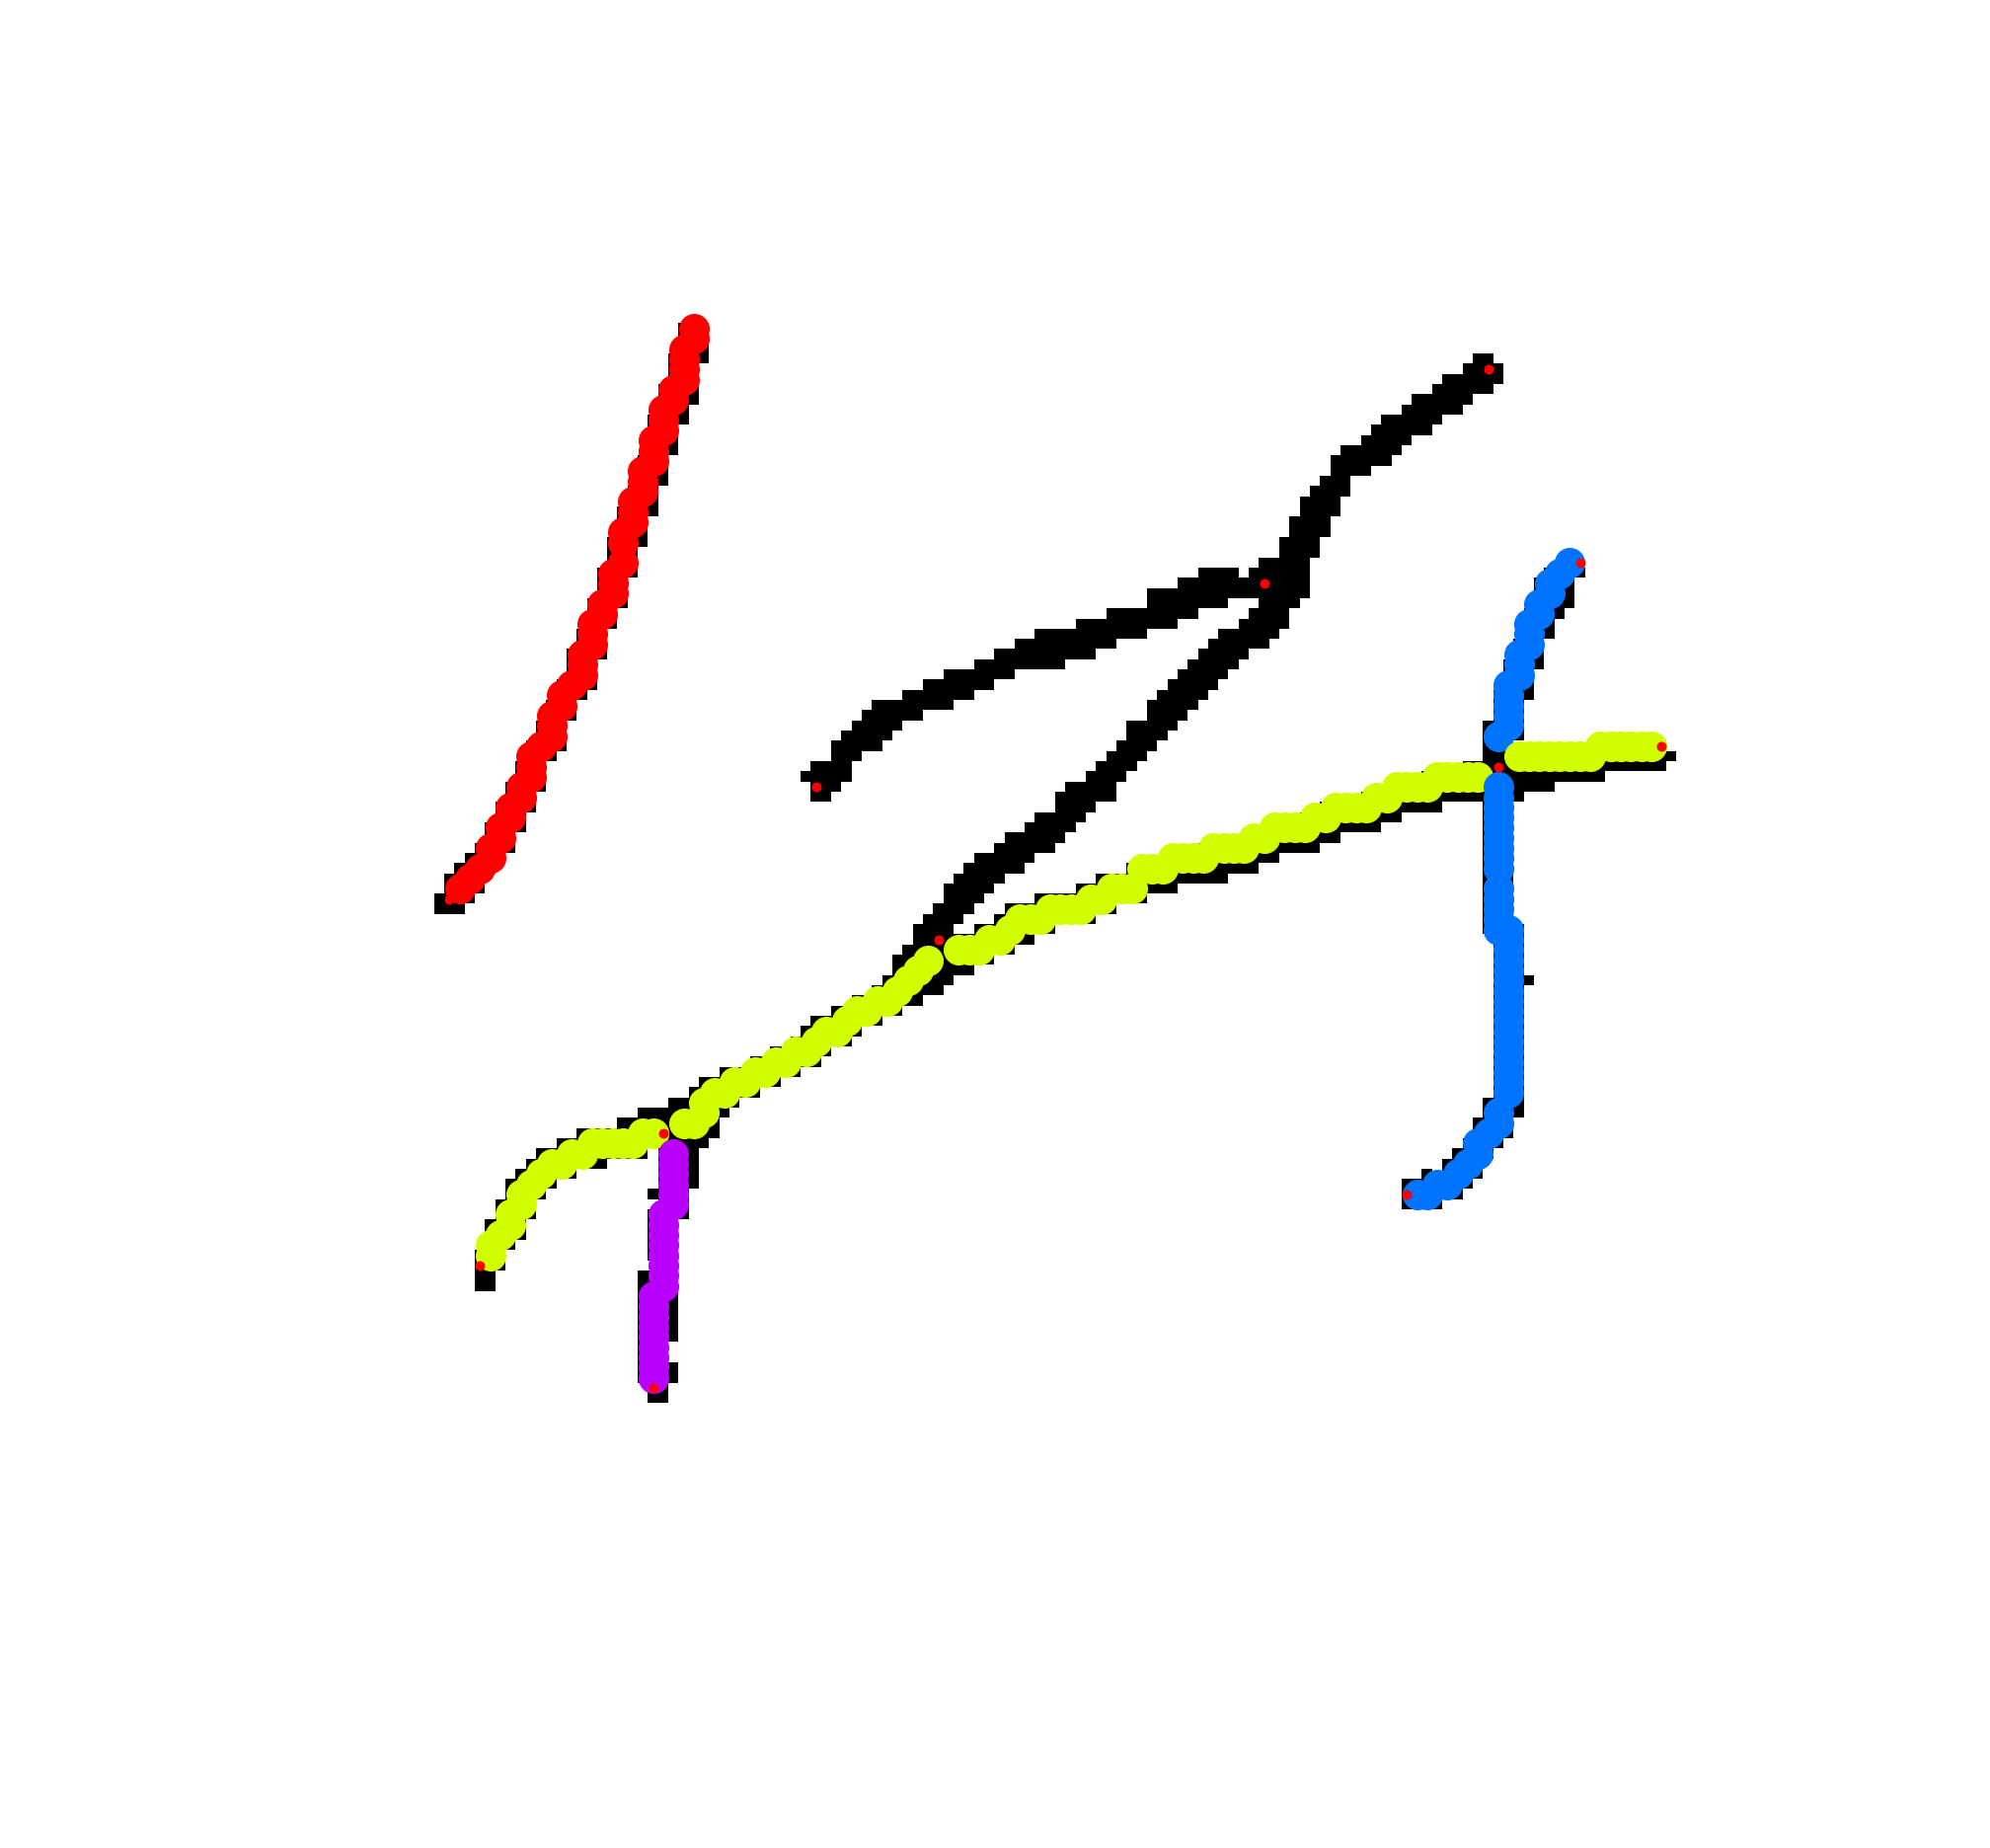
\includegraphics[height=1.3in]{Pictures/Synth-QuantitativeIFS-Fig7-phil-s1271-v056-exactMatch-antLabeled.png}
%         \end{subfigure}
%     \end{figure*}
    
% \resizebox{\textwidth}{!}{
%         %\footnotesize
%         \begin{tabular}{|c|c|c|c|c|c|c|c|c|c|c|c|c|}
%         \hline
%             Config & Iters & P & P* & R & R* & F1 & F1* & C/P & C/P* & C/GT & C/GT* & T[s]\\ \hline
%              DeFiNe 30\textdegree  & 1 & 0.72 & - & 0.47 & - & 0.57 & - & 4/6 & - & 4/6 & - & 2.3 \\
%              DeFiNe 60\textdegree & 1 &0.63 & - & 0.58 & - & 0.60 & - & 3/5 & - & 3/6 &- & 2.3\\
%             AP MT-P & 5 & 0.51 & 0.57 & 0.32 & 0.57 & 0.39 & 0.57 & 3/6.2 & 3/5 & 3/6 & 3/6 & 0.3\\
%             %Mejor Iteraci\'on P1 & 0.5714 & 0.5714 & 0.5714 & 3/5 &  & 0.3135 \\
%             AP S1 & 5 & 0.68 & 0.87 &0.57 & 1 & 0.62 & 0.93 & 4/5.8 & 4/5 & 4/6 & 4/6 & 0.2\\
%             % {\bf Mejor Iteraci\'on P2} & 0.875 & 1 & 0.9333 & 4/5 & 4/6 & 0.3073\\
%              \hline
%         \end{tabular}
%     }
% \end{frame}

\begin{frame}{Im\'agenes Sint\'eticas (OE 4)}

    \begin{columns}
        \begin{column}{0.31\textwidth}
        \vspace{-0.5cm}
            \begin{figure}
                \centering
                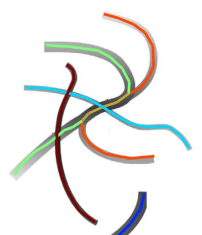
\includegraphics[height=1.3in]{Pictures/define-weighted-4-groundTruth.png}
                \caption{Ground Truth}
            \end{figure}
        \end{column}
        \begin{column}{0.31\textwidth}
        \vspace{-1cm}
            \begin{figure}
                \centering
                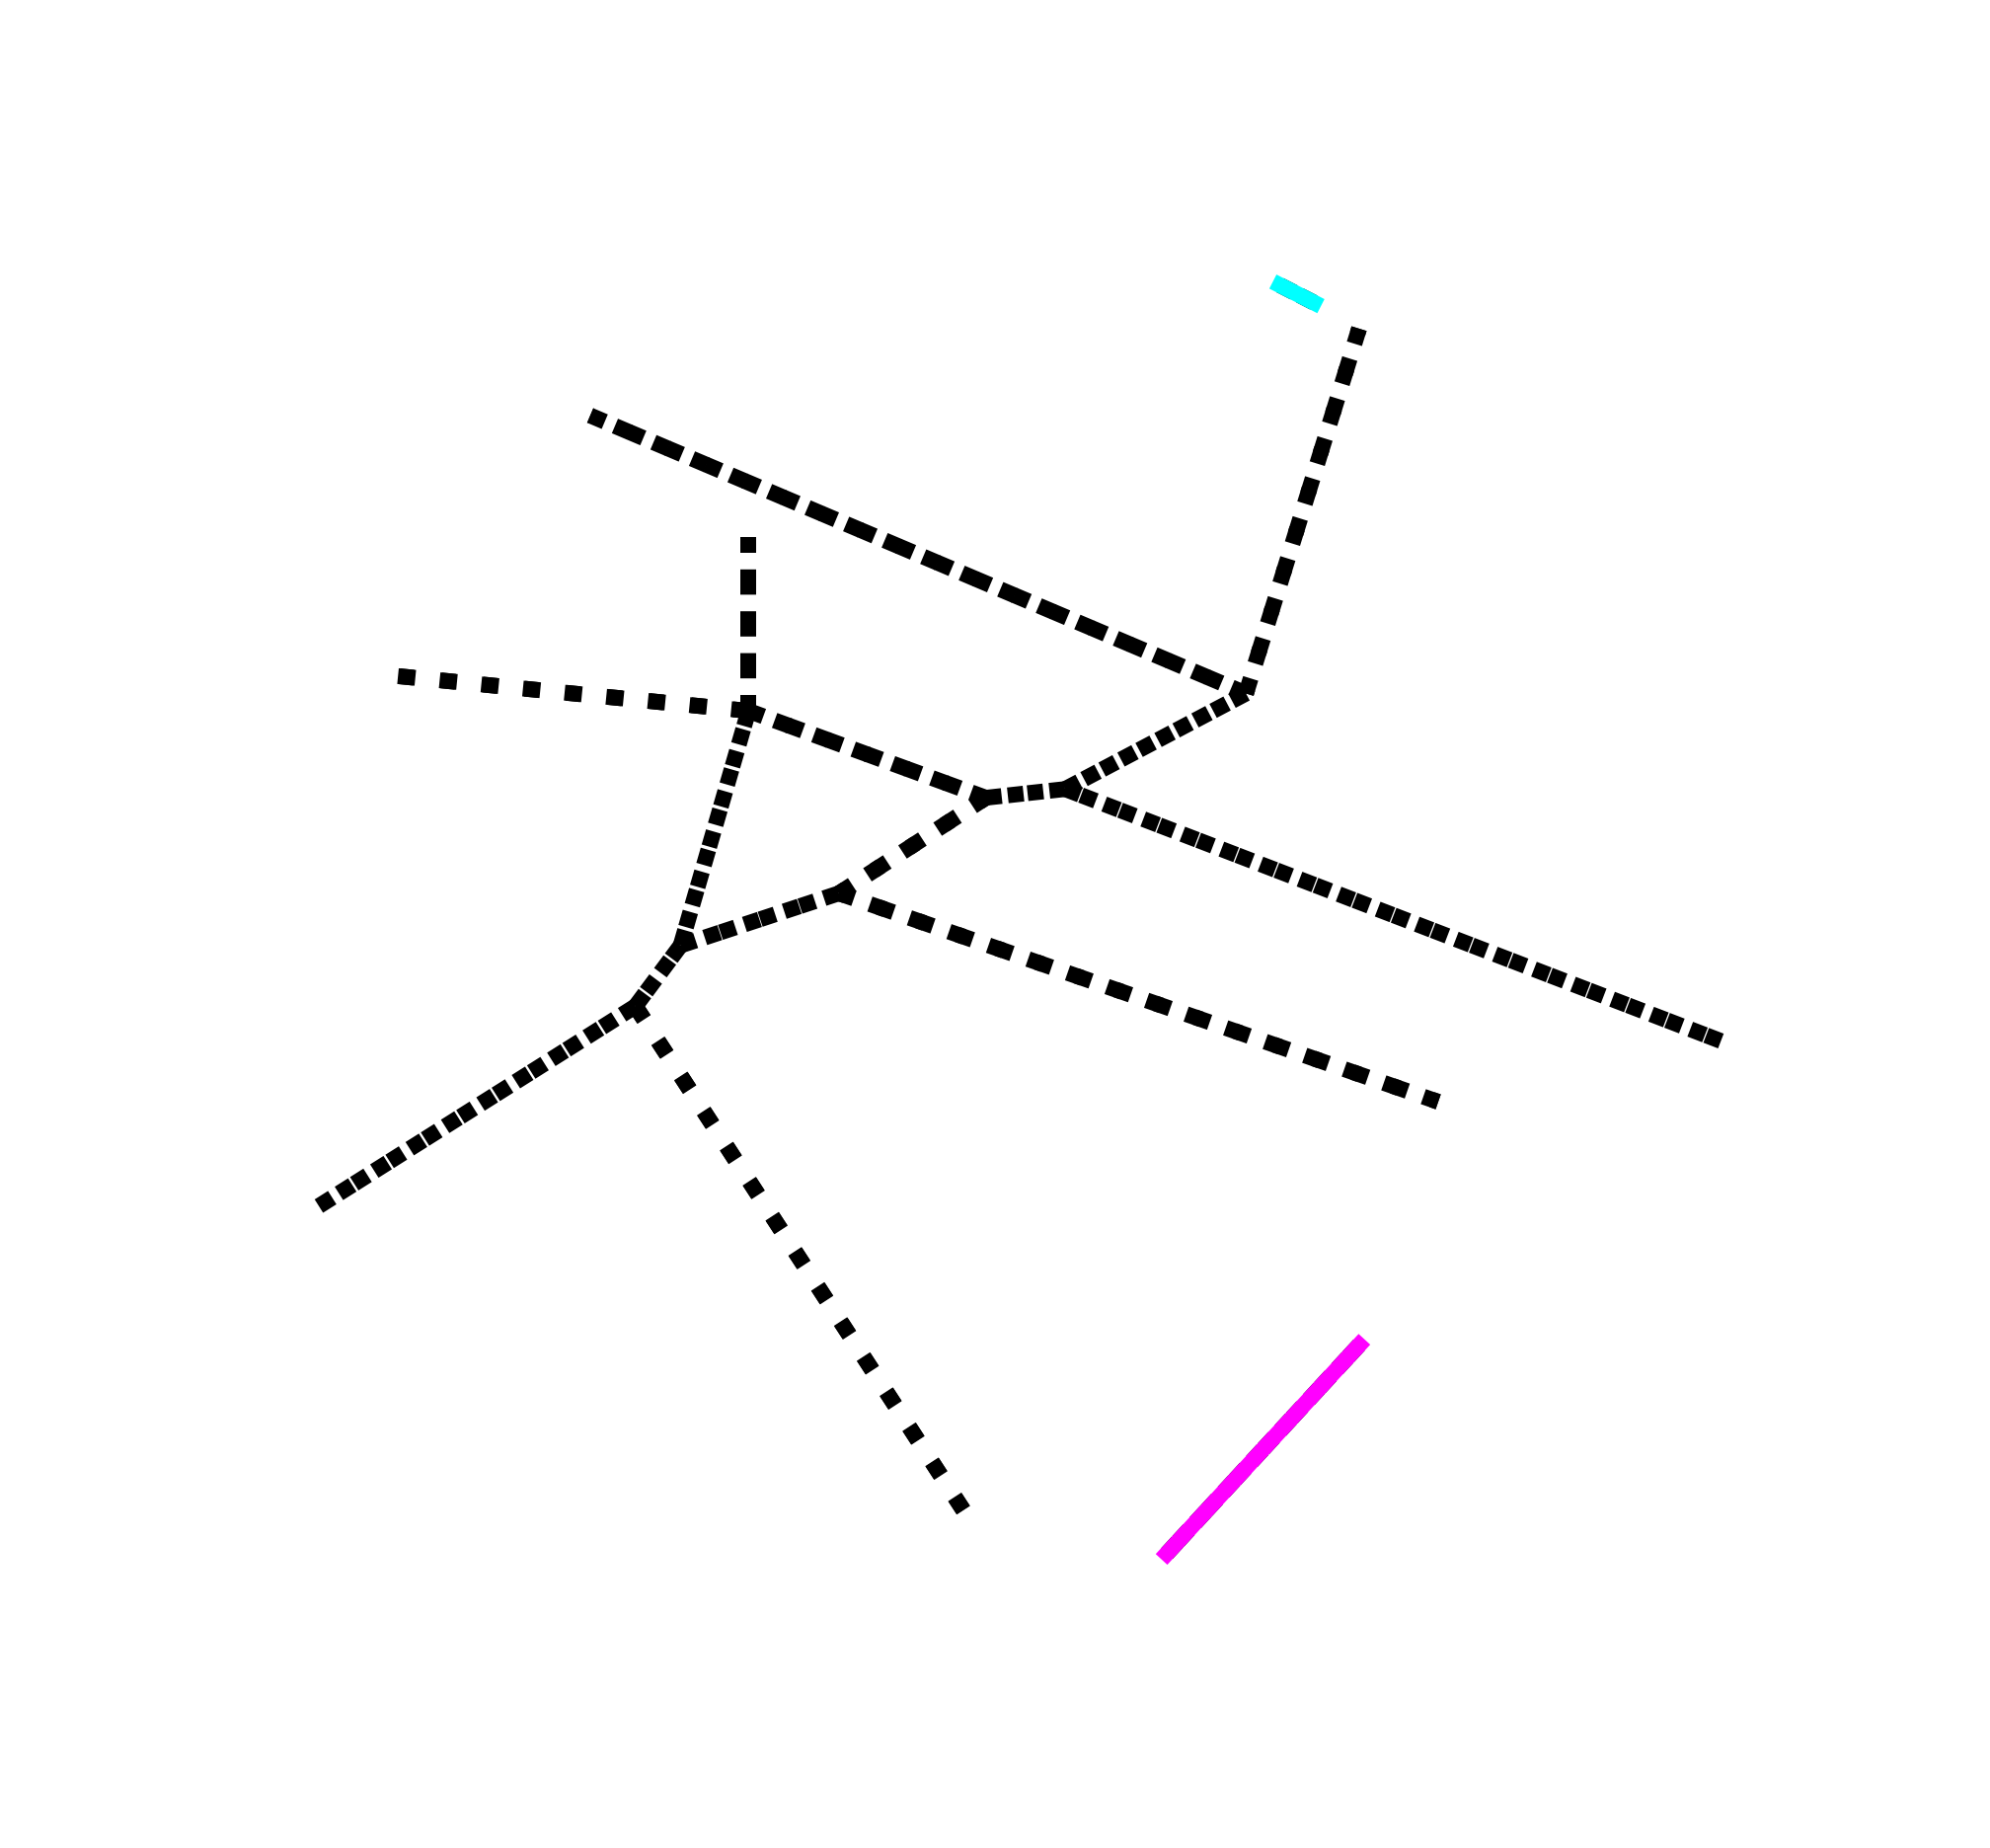
\includegraphics[height=1.3in]{Pictures/defineFig1b-DeFiNeExactMatch-30.png}
                \caption{DeFiNe 30\textdegree}
            \end{figure}
        \end{column}
        \begin{column}{0.31\textwidth}
        \vspace{-1cm}
            \begin{figure}
                \centering
                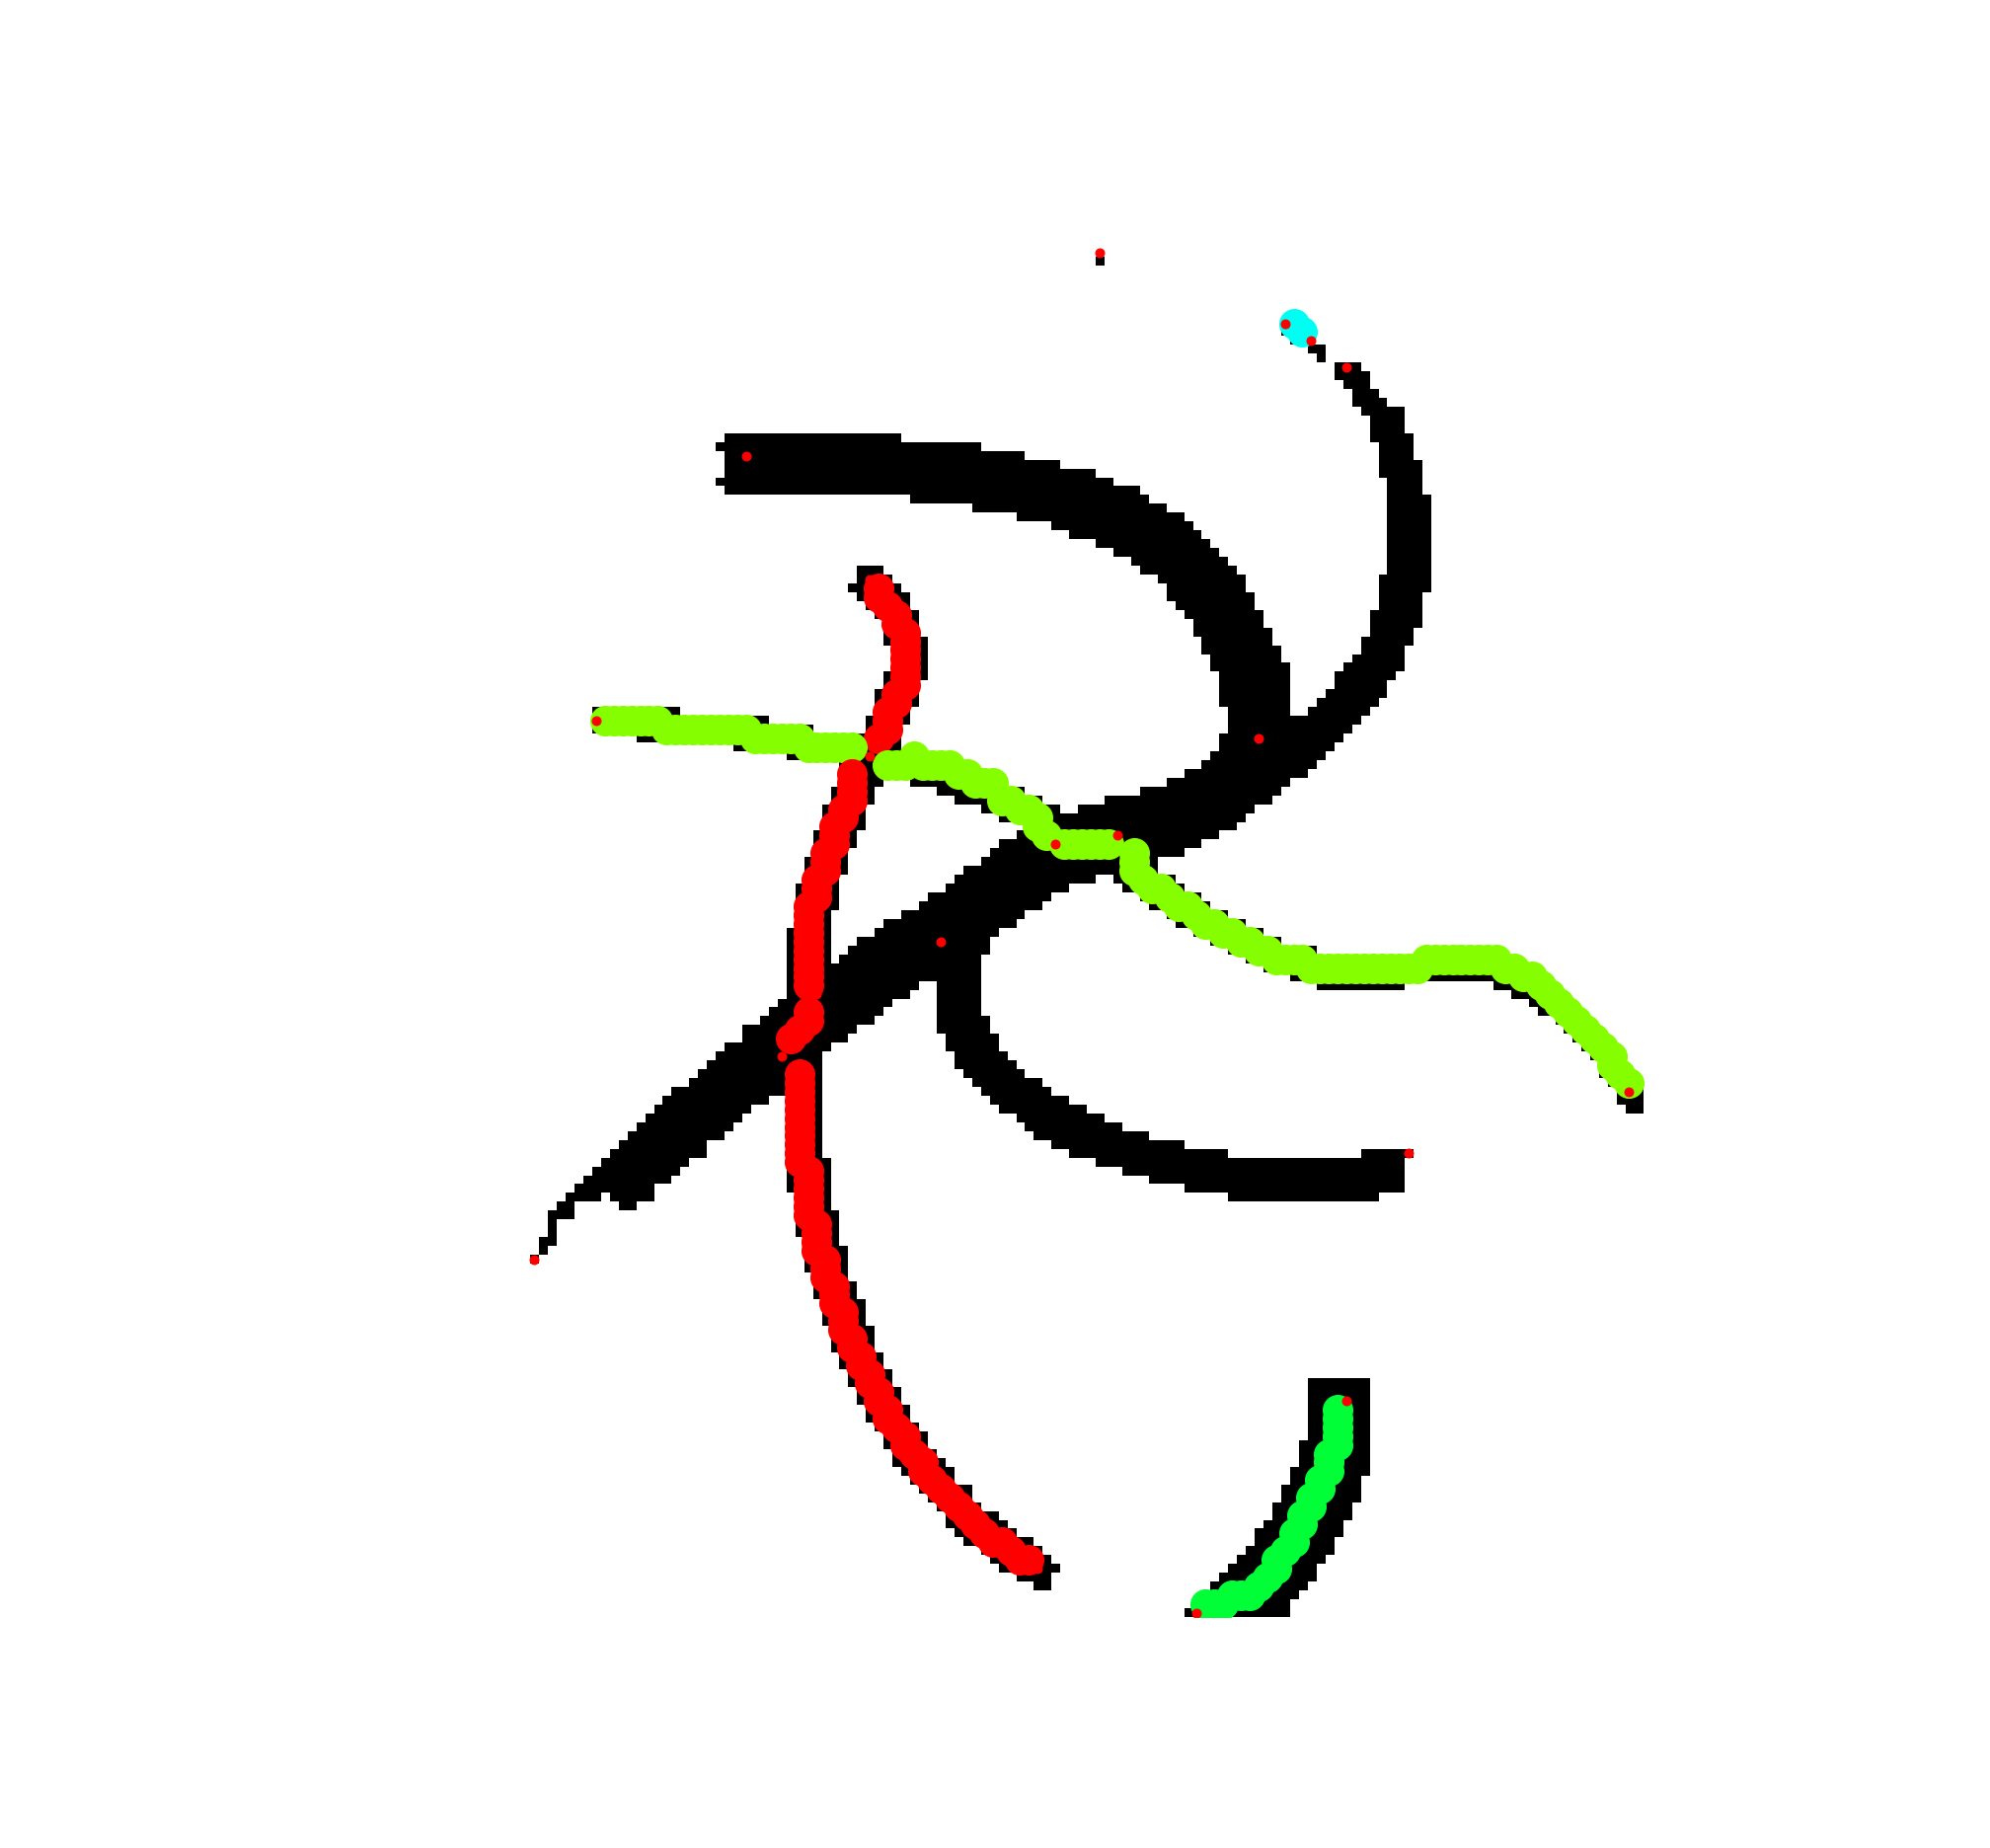
\includegraphics[height=1.3in]{Pictures/define-weighted-4-phil-s3389-v056-exactMatch-antLabeled.png}
                \caption{AP S2}
            \end{figure}
        \end{column}
    \end{columns}

    
    \begin{table}[h]
    \resizebox{\textwidth}{!}{
        \begin{tabular}{|c|c|c|c|c|c|c|c|c|c|c|c|c|}
        \hline
        Config & Iters & P & P* & R & R* & F1 & F1* & C/P & C/P* & C/GT & C/GT* & T[s] \\ \hline
        DeFiNe 30\textdegree & 1 & 0.33 & - & 0.18 & - & 0.23 & - & 2/11 & - & {\bf 2/5} & - & 2.8 \\
        DeFiNe 60\textdegree & 1& 0.23 & - & 0.25 & - & 0.24 & - & 2/7 & - & 2/5 & - & 3.6\\
        AP MT-P & 5 & 0.34 & 0.35 & 0.27 & 0.28 & 0.3 & 0.31 & 3/9.2 & 3/9 & 3/6 & 3/6 & 0.3\\
        AP S2 & 5 & 0.32 & 0.33 & 0.25 & 0.31 & 0.28 & 0.32 & 4/8.6 & 4/9 & {\bf 4/6} & 4/6 & 0.3\\
            \hline
        \end{tabular}
    }
    \caption{Grafo de 17 aristas \\(*) indica el mejor resultado de las 5 iteraciones.}
    \end{table}
\end{frame}

\begin{frame}{Muestra MT-A Microt\'ubulo (OE 4)}
\vspace{-1cm}
    \begin{columns}
        \begin{column}{0.22\textwidth}
            \begin{figure}
                \centering
                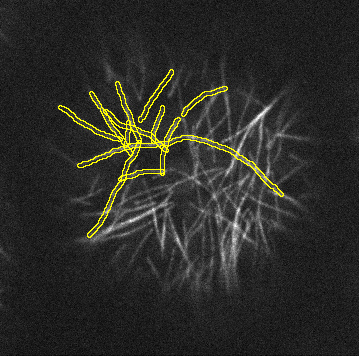
\includegraphics[height=1.3in]{Pictures/SPINNING-DISK-MARCHANTIA-rois-unlabeled.png}
                \caption{Imagen Original}
            \end{figure}
        \end{column}
        \begin{column}{0.22\textwidth}
            \begin{figure}
                \centering
                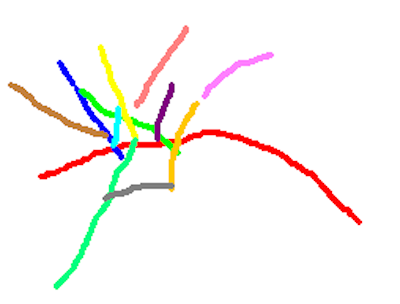
\includegraphics[height=1.3in]{Pictures/50-ROIs-Spinning-Marchantia-solved-rot-unlabeled.png}
                \caption{Ground Truth}
            \end{figure}
        \end{column}
        \begin{column}{0.22\textwidth}
            \begin{figure}
                \centering
                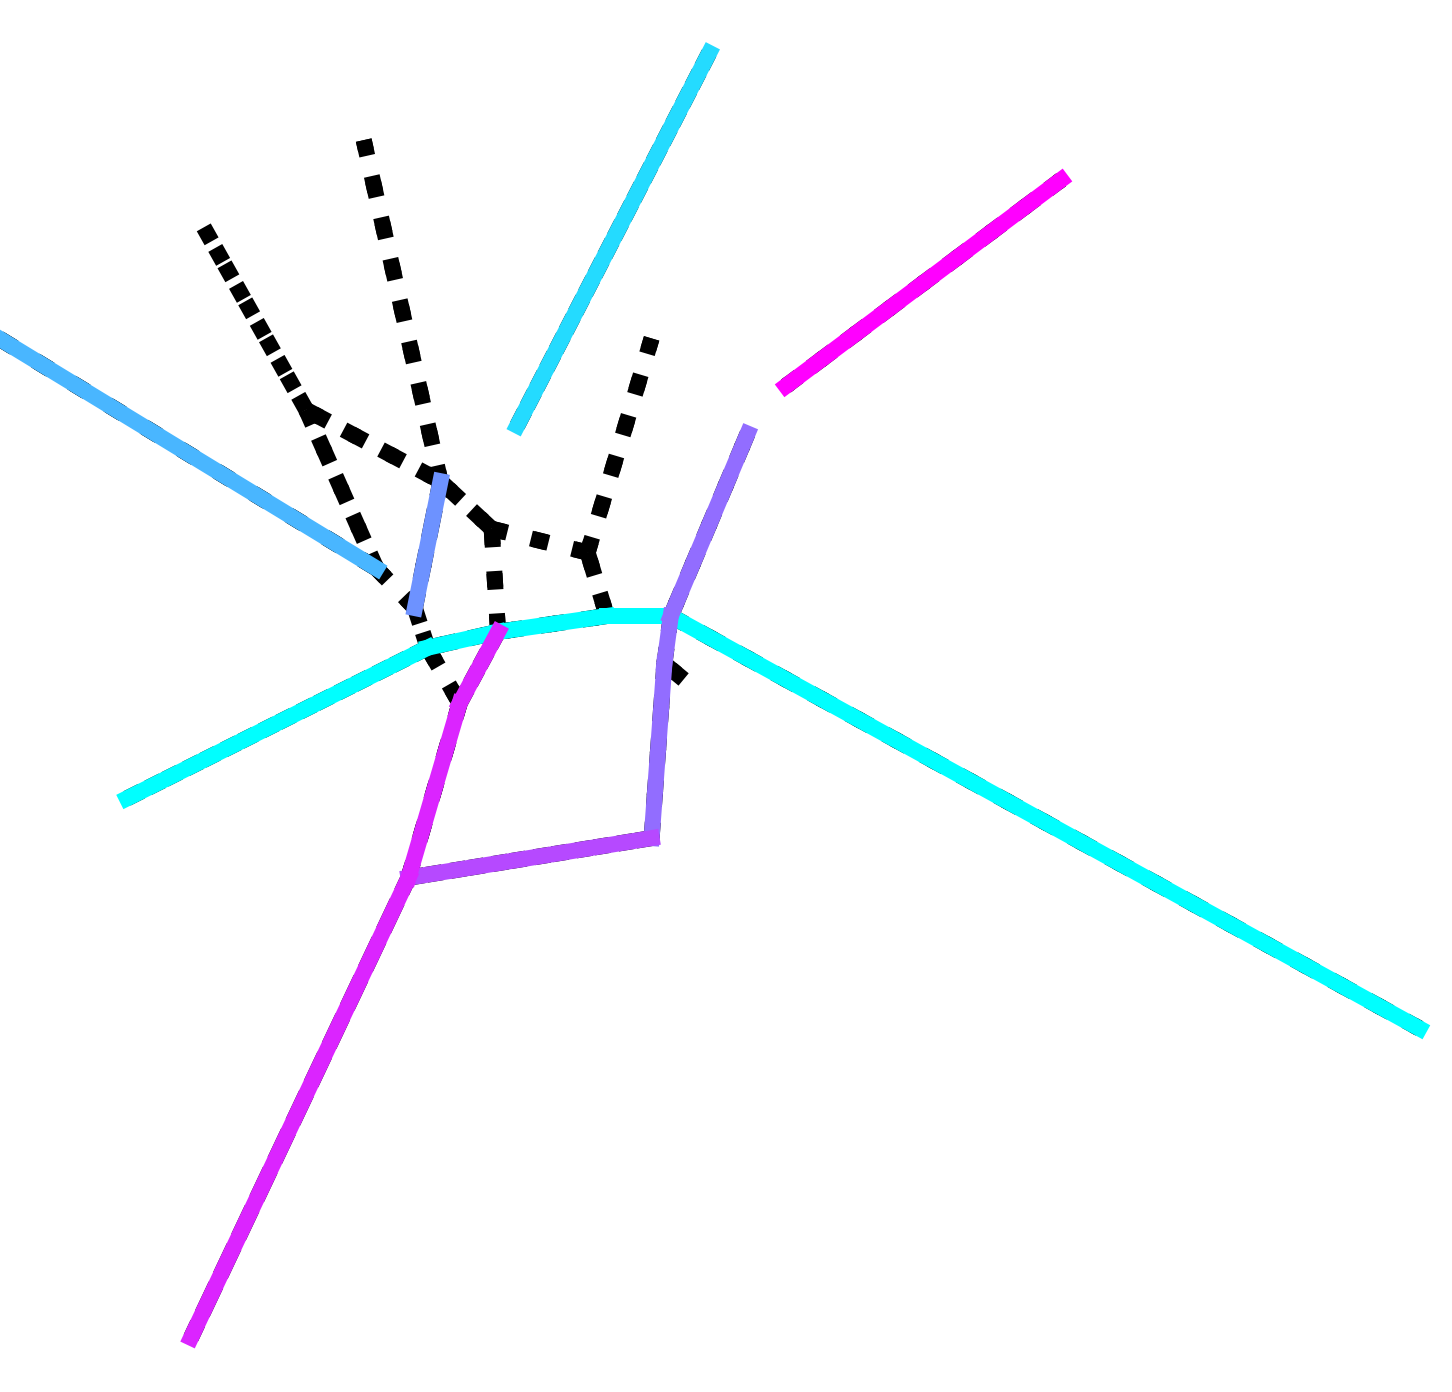
\includegraphics[height=1.3in]{Pictures/50-ROIs-Spinning-Marchantia-DeFiNeExactMatch-30.png}
                \caption{DeFiNe 30\textdegree}
            \end{figure}
        \end{column}
        \begin{column}{0.22\textwidth}
            \begin{figure}
                \centering
                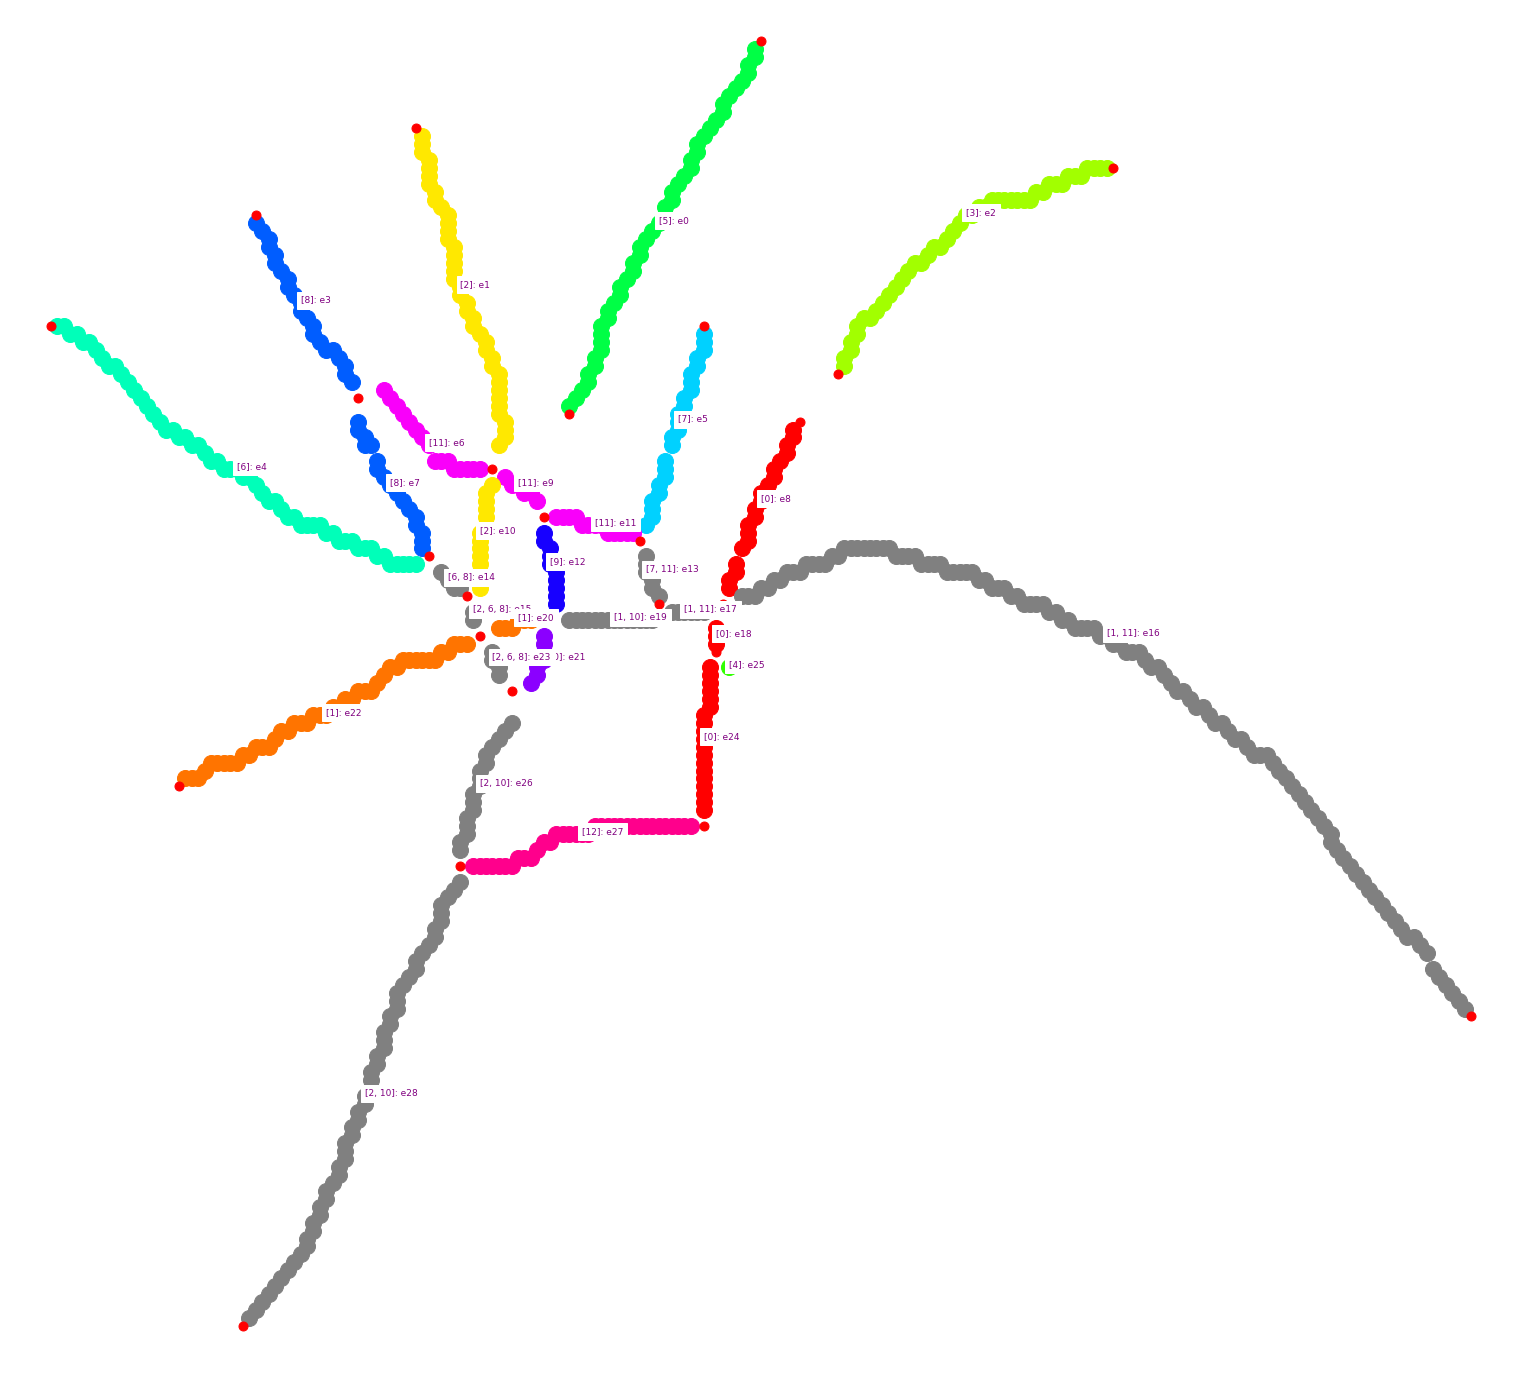
\includegraphics[height=1.3in]{Pictures/50-ROIs-Spinning-Marchantia-phil-s10-v05-nobg-antLabeled.png}
                \caption{AP S2}
            \end{figure}
        \end{column}
    \end{columns}

    \begin{table}[h]
    \resizebox{\textwidth}{!}{
        \begin{tabular}{|c|c|c|c|c|c|c|c|c|c|c|c|c|}
        \hline
              Config & Iters & P & P* & R & R* & F1 & F1* & C/P & C/P* & C/GT & C/GT* & T[s] \\ \hline
             DeFiNe 30\textdegree & 1 & 0.65 & - & 0.45 & - & 0.53 & - & 8/16 & - & {\bf 8/12} & - & 4.1 \\
             DeFiNe 60\textdegree & 1& 0.28 & - & 0.21 & - & 0.24 & - & 3/12 &- & 3/12 & - & 3.6\\
            AP MT-P & 5 & 0.44 & 0.45 & 0.34 & 0.35 & 0.38 & 0.4 & 7.2/12.4 & 8/13 & 7.2/12 & {\bf 8/12} & 0.3\\
             \hline
        \end{tabular}
        }
    \caption{Grafo de 29 aristas \\(*) indica el mejor resultado de las 5 iteraciones}
    \end{table}
\end{frame}

\begin{frame}{Neuronas de rat\'on (OE 4)}
\vspace{-1cm}
    \resizebox{\textwidth}{!}{
        \begin{tabular}{|c|c|c|c|c|r|c|}
        \hline
             Muestra & Algoritmo & Fil. Propuestos & {\it GT} &\% Asignaci\'on & Tiempo[s] & N\textdegree~ Aristas\\
             \hline
             \multirow{3}{*}{N1}& DeFiNe 30\textdegree & 246 & \multirow{3}{*}{24} &100 & 1514.6 & \multirow{3}{*}{414} \\
                    & DeFiNe 60\textdegree & 192 && 100 & 15573.7 &\\
                    & AP N Promedio & 59 && 53.7 & 32.5 &\\ \hline
            \multirow{3}{*}{N2}& DeFiNe 30\textdegree & 113 & \multirow{3}{*}{29} & 100 & 82.2 & \multirow{3}{*}{161}\\
                    & DeFiNe 60\textdegree & 85 && 100 & 456.4 &\\
                    & AP N Promedio & 34.8 && 59.3 & 4.9 &\\ \hline
            N3 & AP N Promedio & 17.4 & 14 & 57.8 & 4.2 & 67\\ \hline
        \end{tabular}
    }
    \vspace{1cm}
    \begin{itemize}
        \item \% Asignaci\'on debe estar relacionado a la calidad de la informaci\'on, evitando asignar s\'olo por cumplir con el modelo
        \item N\textdegree~ Fil. Prop. refleja acotamiento del espacio de b\'usqueda
    \end{itemize}
\end{frame}

\begin{frame}{Muestra N3 de neurona de rat\'on (OE 4)}
    \vspace{-1cm}
        \begin{columns}
        \begin{column}{0.45\textwidth}
            \begin{figure}
                \centering
                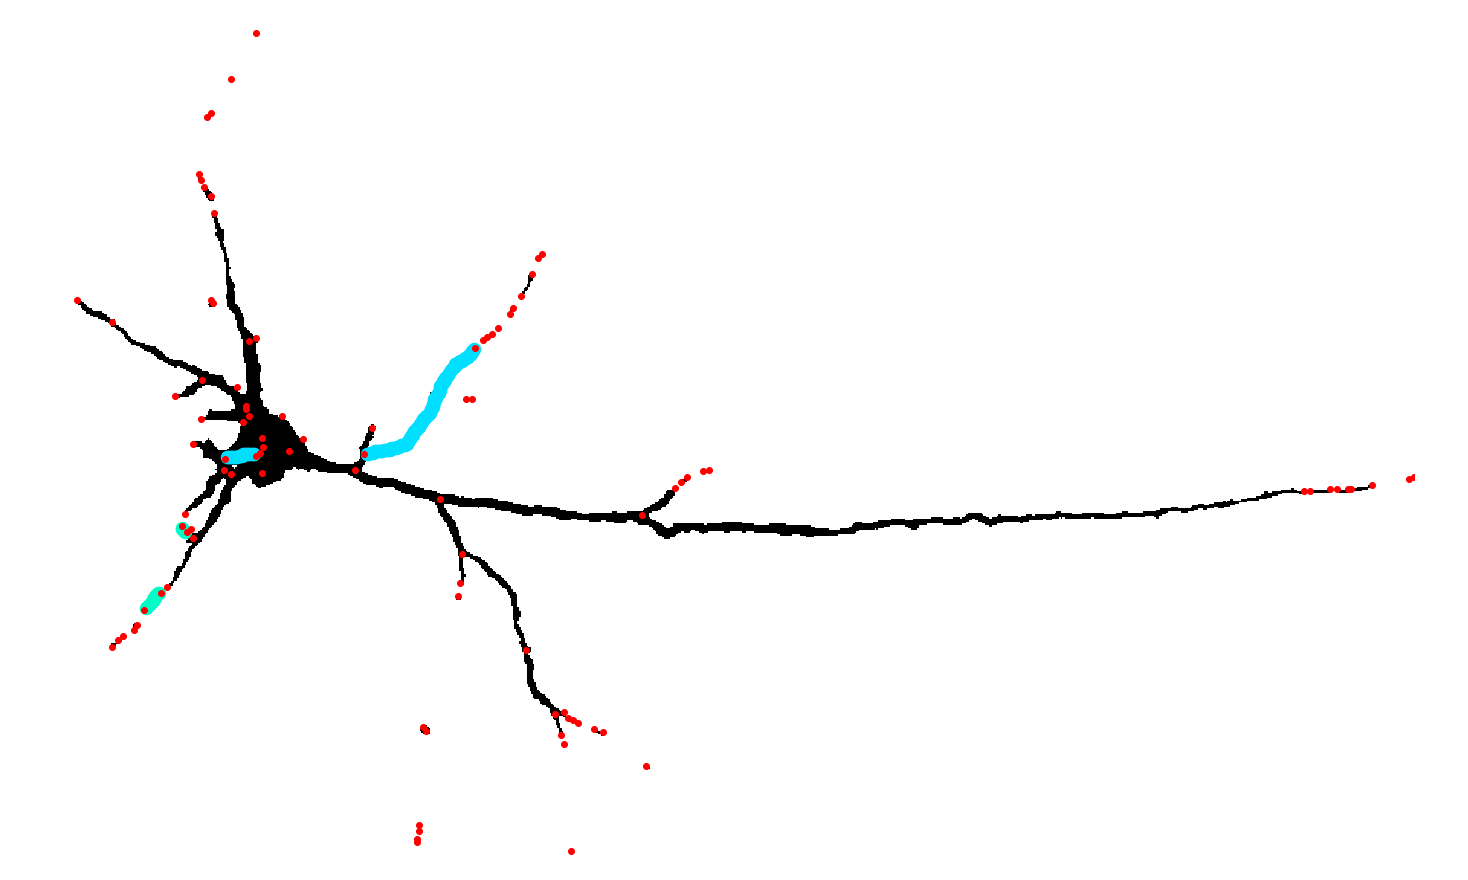
\includegraphics[height=1.3in]{Pictures/Porta18-3a1-phil-s10-v056-exactMatch-antLabeled.png}
                \caption{Muestra N3 Calce Exacto}
            \end{figure}
        \end{column}
        \begin{column}{0.45\textwidth}
            \begin{figure}
                \centering
                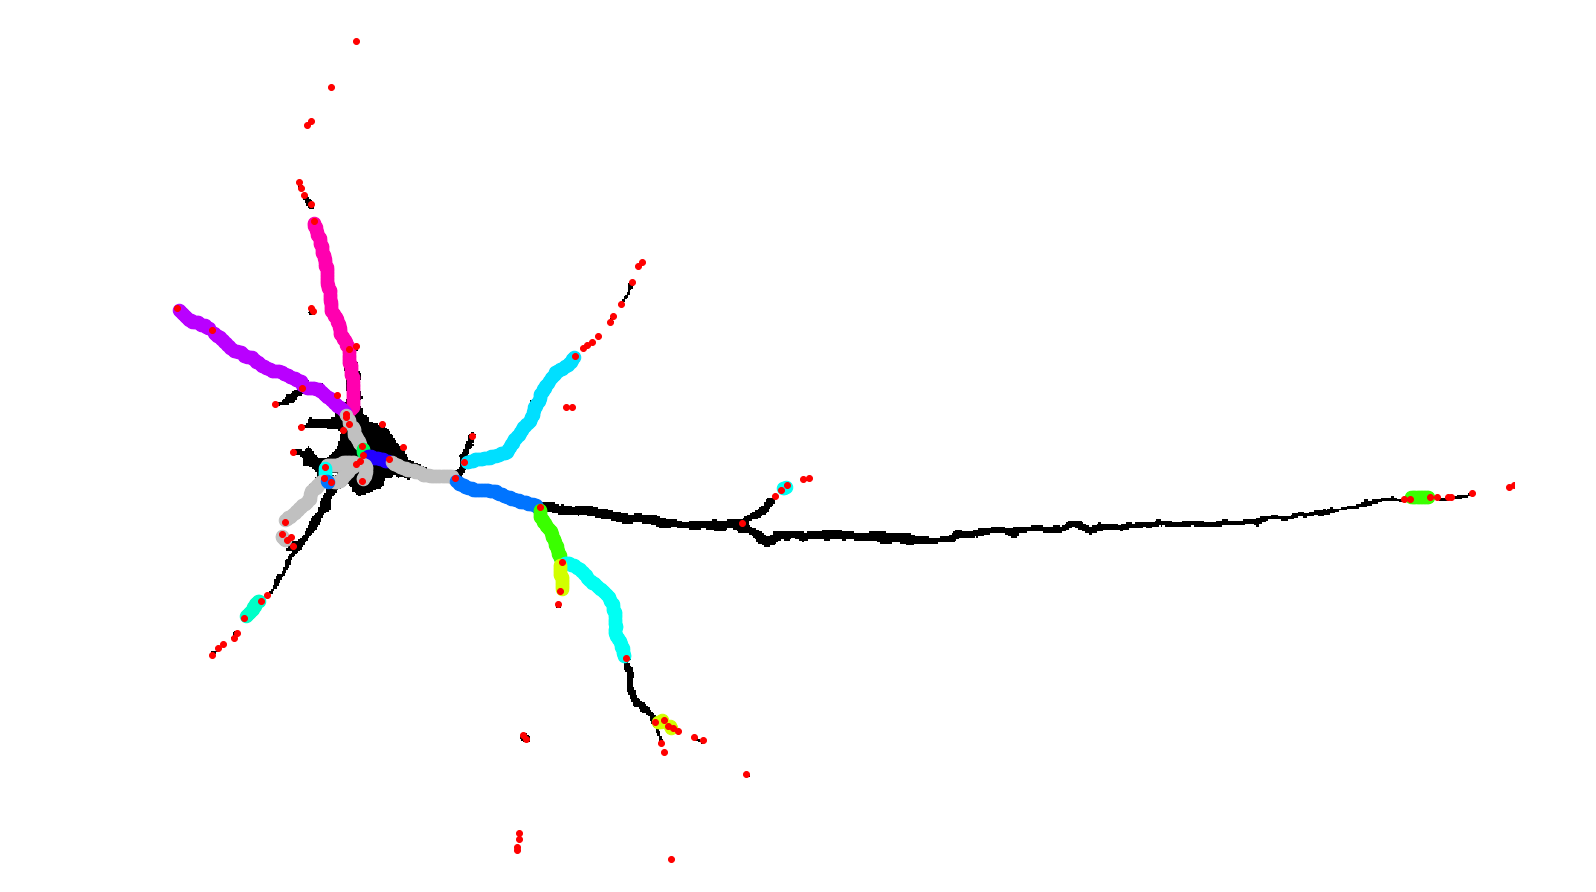
\includegraphics[height=1.3in]{Pictures/Porta18-3a1-phil-s10-v056-overmatches-3-antLabeled.png}
                \caption{Muestra N3 con sub/sobre asignaci\'on}
            \end{figure}
        \end{column}
    \end{columns}
    
    \begin{table}[h]
    \resizebox{\textwidth}{!}{
        \begin{tabular}{|c|c|c|c|c|c|c|c|c|c|c|c|c|}
        \hline
              Muestra & P & P* & R & R* & F1 & F1* & C/P & C/P* & C/GT & C/GT* & F.S. & F.S.* \\ \hline
            N1 & 0.62 & 0.6 & 0.15 & 0.13 & 0.24 & 0.22 & 1.6/59 & 3/66 & 1.6/24 & 3/24 & 1.4 & 1\\
            N2 & 0.2 & 0.21 & 0.09 & 0.1 & 0.13 & 0.14 & 4.6/34.8 & 6/34 & 4.6/29 & 6/29 & {\bf 8} & 7 \\
            N3 & 0.5 & 0.47 & 0.32 & 0.29 & 0.39 & 0.36 & 2/17.4 & 2/17 & 2/14 & 2/14 & {\bf 7.8} & 8\\
            \hline
        \end{tabular}
        }
        \caption{(*) indica el mejor resultado de las 5 iteraciones}
    \end{table}
\end{frame}

\begin{frame}{Resultados Generales (OE 4)}
\resizebox{\textwidth}{!}{
    \begin{tabular}{|c|c|c|c|c|c|}
        \hline
        & &                 Filamentos & Promedio Filamentos & Distribuci\'on &   \\
        Figura & Configuraci\'on & Correctos & Propuestos 10 Iters & Normal & $p$-value  \\ \hline
         4.1 & S1  & 6 & 5.9 & No & {\bf 1} \\
         4.2 & S2 & 5 & 8.5 & No & 0.003\\
         4.3 & MT-P & 12 & 12.4 & No & {\bf 0.125}\\
         4.4 & MT-P & 12 & 15 & Si & 0\\
         4.5 & MT-P & 5 & 5 & No & {\bf 1}\\
         4.6 & N & 24 & 60.2 & Si & 0\\
         4.7 & N & 29 & 34.3 & Si & 0\\
         4.8 & N & 14 & 17.6 & No & 0.003\\ \hline
    \end{tabular}
}
    % \begin{itemize}
    %     \item Comparaci\'on de conjuntos ofrece menos claridad que comparaci\'on por clasificaci\'on
    % \end{itemize}
\end{frame}